\documentclass[]{scrartcl}
\title{Vorlesung Analysis II}
\usepackage{amsmath,amssymb,amsfonts}
\usepackage{mathtools}
\usepackage{latexsym}
\usepackage{graphicx}
\usepackage{tikz}
\usepackage{xcolor}
\usepackage{soul}
\usepackage{hyperref}
\usepackage{tipa}
\hypersetup{
	colorlinks=true,
	linkcolor=blue,
	filecolor=magenta,      
	urlcolor=cyan,
	pdftitle={Overleaf Example},
	pdfpagemode=FullScreen,
}
\newcommand{\redcircle}[1]{%
	\tikz[baseline=(char.base)]{
		\node[shape=circle, draw=red, text=red, thick, inner sep=1pt] (char) 
		{\textbf{#1}};
	}%
}
\setul{1pt}{1.5pt} % Linienhöhe und Abstand zum Text (optional anpassbar)

\setlength{\topmargin}{-.5in} \setlength{\textheight}{9.25in}
\setlength{\oddsidemargin}{0in} \setlength{\textwidth}{6.8in}
\setlength{\parindent}{0pt}

\begin{document}
\maketitle
\textbf{\underline{Teil 1: Differnetialrechnung im $\mathbb{R}^n$}}\\
\\
\textbf{\underline{an2: Geometrie von Funktionen 
$\mathbb{R}^n\rightarrow\mathbb{R}^m$ 
mit m=1 und n=1}}\\
\textbf{\underline{Stichworte:}}Affine Räume, Parameter- und 
Normalendarstellung, 
Funktionen 
$\mathbb{R}^n\rightarrow\mathbb{R}^m$\\
\textbf{\underline{Literatur:}}\setulcolor{blue} \ul{[Hoff], Kapitel 9.2}\\
\\
\textbf{2.1}\underline{\textbf{Einleitung}}: Nach Kurzer Überlegung zur 
Darstellung 
affin-Linearer Objekte im $\mathbb{R}^n$, also Geraden, Ebenen, Hyperebenen,... 
arbeiten wir an der geometrischen Anschauung von Funktionen 
$f:\mathbb{R}^n\rightarrow\mathbb{R}^m$, die affinlinear oder nicht affinlinear 
sind. Wir betrachten insbesondere $\mathbb{R}$-wertiger (auch: reellwertiger)\\
Funktionen, d.h. solche Funktionen $f:\mathbb{R}^n\rightarrow\mathbb{R}$ mit n 
= 1, sowie auch "Kurvenartige Funktionen $f: 
\mathbb{R}\rightarrow\mathbb{R}^m$ mit m = 1.\\\\
\textbf{2.2\underline{Affine Räume}} im $\mathbb{R}^n$: Ist 
$U\subseteq\mathbb{R}^n$ ein 
Untervektorraum des $\mathbb{R}^n$, so heißt a+U für ein $a\in \mathbb{R}^n$ 
ein (d-dimensionaler) \setulcolor{red} \ul{affiner Raum}, wenn dim U=d ist. 
(Man kann a einen \ul{Aufpunkt} von a+U nennen.)\\
Es gibt folgende Arten zur Beschreibung der El. von a+U:\\
\textbf{2.3 $\bullet$\underline{Parameterdarstellung:}} \ul{Ist u die} Lineare 
Hülle von 
Vektoren $v_1,...,v_r$, d.h. U= L$(v_1,...,v_r) : = \{\alpha_1 v_1+...+\alpha_r 
v_r; \alpha_1,...,\alpha_r\in\mathbb{R}\} = \mathbb{R}v_1+...+\mathbb{R}v_r$, 
d.h. die Menge aller Linearkombinationen $\sum_{i=1}^{r}\alpha_i v_i$ der 
$v_1,...,v_r$, auch: der \ul{Span} der $v_1,...,v_r$ geschrieben 
\setulcolor{yellow} \ul{$span(v_1,...,v_r)$},\\
bzw. auch: das \setulcolor{red} \ul{Lineare Erzeugnis} der $v_1,...,v_r$ 
geschrieben$\textless v_1,...,v_r\textgreater$($\leftarrow$ keine 
skalarproduktklammern, sondern "Erzeugnissklammern"!)\\
Dann ist a+U = a+L($v_1,...,v_r) = \{a+\alpha_1 v_1 +...+ \alpha_r v_r; 
\underbrace{\alpha_1,...,\alpha_r\in \mathbb{R}}_{\textbf{die Parameter}}\}$\\

Sind $v_1,...,v_r$ Linear unabhängig, gilt dim(a+U)=dim U = r, die 
$v_1,...,v_r$ heißen dann \ul{Richtungsvektoren}.\\
Für r= dim U = 1 ist die eine \ul{Gerade} $a + \mathbb{R}v_1 = \{a+tv_1; 
t\in\mathbb{R}^n\}$, "in Richtung" $v_1\in \mathbb{R}^n, v_1\neq 0$, und mit 
Aufpunkt $a \in \mathbb{R}^n$. Für r=dim U = 2  ist dies eine \ul{Ebene} $a + 
\mathbb{R}v_1 + \mathbb{R}v_2 = \{a+tv_1+sv_2; t,s \in 
\mathbb{R}\}\subseteq\mathbb{R}^n$ mit zwei (linear unabh.) Richtungsvektoren 
$v_1,v_2\in \mathbb{R}^n$ und Aufpunkt $a\in \mathbb{R}$. Usw.\\
Eine besonders einfache Darstellung ist im Fall dim U = n-1 möglich, den 
zugehörigen affinen Raum nennen wir eine \ul{Hyperebene in $\mathbb{R}^n$}:\\
\\
\textbf{2.4$\bullet$ \underline{Normalendarstellung}}(einer \ul{Hyperebene} im 
$\mathbb{R}^n$):\\
Sei \setulcolor{yellow} $H_{c,a}:=\{x\in\mathbb{R}^n|\textless x,c\textgreater 
= \alpha\}$ für $c \in \mathbb{R}^n, c\neq 0,$ und $\alpha \in \mathbb{R}.$\\
Sei $p\in H_{c,\alpha}$ irgendein Punkt dieser Menge, d.h. es gelte $\textless 
p,c \textgreater = \alpha$.\\
Dann ist $H_{c,\alpha} = p+U$ mit einem Untervektorraum $U\subseteq  \mathbb{R}^n$, für den dim U = n-1 ist, denn: $U=ker f$ für die Lineare Abb. $f:\mathbb{R}^n \rightarrow \mathbb{R}, x \rightarrow\textless x,c\textgreater\\
$\textopencorner$ x \in H_{c,\alpha}\Leftrightarrow \textless x,c \textgreater = \alpha \Leftrightarrow\textless x-p,c \textgreater = \alpha - \textless \underbrace{\textless p,c \textgreater}_{\alpha} \Leftrightarrow x = p+n$ mit $ n \in ker f $\textcorner\\
dabei ist  $imf=\mathbb{R}$, also $dim U= dim ker f = n - dim imf =n-1$\\
Mit U = ker f $=\{u \in \mathbb{R}; \textless u,c \textgreater = 0\} =: \{c\}^{\bot}$ folgt, dass die $u\in U$ genau die Vektoren im $\mathbb{R}^n$ sind, die senktrecht auf c stehen, bzw. wir haben \setulcolor{green} \ul{$U^{\bot}=\mathbb{R}c$}.\redcircle{Ü}\\
Da c senkrecht zu jedem Punkt von U ist, heißt c \setulcolor{red}\ul{Normalenvektor} von $H_{c,\alpha}$.
Denn eine Gerade $p+\mathbb{R}c\subseteq \mathbb{R}^n$
 heißt \ul{Normale} von $H_{c,\alpha}$ und steht senkrecht auf $H_{c,a}$.\\\\
\textbf{2.5} $\bullet$ Ein Spezialfall der Normalendarstellung ist die 
\ul{Hessesche Normalform:} $H_{c,\alpha}$ mit \ul{$||c|| = 1$} (wo der 
Normalenvektor auf 1 normiert ist).\\
 Die Formel in \setulcolor{blue} \ul{2.8 und 2.9} werden dann noch einfacher.\\\\
\textbf{ 2.6 \underline{Bsp. zur Normalendarstellung:}}\\ Eine Ebene E im Raum 
$\mathbb{R}^3$ kann in der Form $E = \{\begin{pmatrix} 
 		\xi_1\\
 		\xi_2\\
 		\xi_3
 \end{pmatrix}; \underbrace{\gamma_1\xi_1+\gamma_2\xi_2+\gamma_3\xi_3}_{=\textless x,c \textgreater}= \alpha\}$ dargestellt werden; c= 
$\begin{pmatrix} 
	\xi_1\\
	\xi_2\\
	\xi_3
\end{pmatrix}$ ist darin der Normalenvektor, d.h. c $\bot$ E.\\
Die Eben $E = \{\begin{pmatrix} 
		x\\
		y\\
		z
\end{pmatrix}\in \mathbb{R}^3; 3x-2y-z=2\}$ z.b. steht senkrecht auf c= $\begin{pmatrix} 
3\\
-2\\
-1\\
\end{pmatrix}$.\\
In dieser Form nennt man die Normalendarstellung auch oft \setulcolor{red} \ul{Koordinatendarstellung} von E. Anderes Bsp.  $E = \{\begin{pmatrix} 
		x\\
		y\\
		z
	\end{pmatrix}\in \mathbb{R}^3; x=0\}$ ist die y-z-Ebene, und  $E = \{(w,x,y,z)\in \mathbb{R}^4; w-3x-y+4z=10\}$ ist die (3-dim) Hyperevene im $\mathbb{R}^4$, die senkrechte zu $\begin{pmatrix}
	1\\
	-3\\
	-1\\
	4
\end{pmatrix}$ ist.\\
\\
\textbf{2.7\underline{Schul bsp. zur Normalendarstellung:}} Eine Gerade g in 
der Ebene $\mathbb{R}^2$ ist auch eine "Hyperebene" im $\mathbb{R}^2$, da dim g 
=1=2-1 gilt.\\
Eine Normalendarstellung lautet dann $g=\{\begin{pmatrix}
		x\\
		y
\end{pmatrix} ;\textless \begin{pmatrix}
x\\
y
\end{pmatrix} ,
\begin{pmatrix}
	\gamma_1\\
	\gamma_2
\end{pmatrix}  \textgreater = \alpha\}$ für $\gamma_1, \gamma_2, \alpha \in \mathbb{R}$, d.h. wird beschrieben durch die Gleichung $\gamma_1 x+ \gamma_2 y = \alpha \Leftrightarrow (\gamma_2 \neq 0) y = -\frac{\gamma_1}{\gamma_2}x + \frac{\alpha}{\gamma_2} \leftarrow$ Geradengleichung der Schule mit Steigung m = $\frac{\gamma_1}{\gamma_2}$, und c =$\frac{\alpha}{\gamma}$ als y-Achsenabschnitt.\\
Sogar an eine "Schulglg." $1\cdot y=mx+c$
 für eine Gerade kann man also den Normalenvektor $\begin{pmatrix}
 	-m\\
 	1
 \end{pmatrix}$ ablesen, der senkrecht auf der Geraden g (mit Richtungsvektor $\begin{pmatrix}
 m\\
 1
 \end{pmatrix}$) steht: $\textless \begin{pmatrix}
 -m\\
 1
 \end{pmatrix}\begin{pmatrix}
 1\\
 m
 \end{pmatrix} \textgreater = -m +m =0$.\\
 \newpage
\textbf{2.8 \underline{Rechen mit der Hesseschen Normalform:}}
 Sei $E= H_{c,\alpha}=\{x\in\mathbb{R}^n;\textless x,c\textgreater=\alpha\}, c\neq0$\\
 1. \underline{Beh.:} $\bullet$ Ist $H_{c,\alpha}\subseteq \mathbb{R}^n$ geg., so ist der Abstand von 0 zu $H_{c,\alpha}$ gegeben als $dist(0,H_{c,\alpha})=\frac{|\alpha|}{||c||}$.\\
 $\bullet$ Ist außerdem $||c||=1$, ist dieser Abstand also =$|\alpha|$.\\
 \underline{Bew.:} Sei $x\in H_{c,\alpha}$ beliebig.
 Der gesuchte Abstand ist die Länge von p(x,c), also $dist(0, 
 H_{c,\alpha})=||p(x,c)||=||\frac{\textless x,c\textgreater}{\textless 
 c,c\textgreater}\cdot c||=\frac{|\textless 
 x,c\textgreater|}{||c||}=\frac{|\alpha|}{||c||}. \square$
 \begin{figure}[h]
 	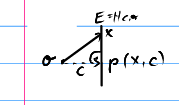
\includegraphics[width=2.5cm,height=2cm]{Beispiel 2.8}
 \end{figure}\\
\underline{Bsp.:} 
$H_{\begin{pmatrix}
	1\sqrt{2}\\
	1\sqrt{2}
\end{pmatrix},-7}=\{\begin{pmatrix}
	x\\y
\end{pmatrix}; \frac{1}{\sqrt{2}}x+\frac{1}{\sqrt{2}}y=-7\}$(hier: 
$||c||=\sqrt{\frac{1}{2}+\frac{1}{2}}=1$) hat den Abstand $\underbrace{|\alpha| = |-7|=7}_{\text{ist nicht der y-Achsenabschnitt!}}$ 
vom Ursprung o.\\
\\
\textbf{2.9 2.\underline{Beh.:}} Ist $H_{c,\alpha}\in \mathbb{R}^n$ geg., so ist 
der 
Abstand von (irgendeinem) $ q \in \mathbb{R}^n$ zu $H_{c,\alpha}$ gegeben als\\
\begin{equation}
	dist(q,H_{c,\alpha})= \frac{|\textless q,c\textgreater-\alpha |}{||c||}.
\end{equation}
\textbf{\underline{Bew.:}} Betr. die um q verschobene Ebene $E'= \{x'; x'+q\in 
E\}$, dann ist der gesuchte Abstand der von 0 zu E', für ein $x'\in E'$ also 
$=||p(x',c)|| = [\rightarrow x'+q=x\in E] ||p(x-q,c)||$\\
\begin{equation}
	=||\frac{\textless x-q,c\textgreater}{\textless c,c \textgreater}\cdot c||=
	||\frac{\textless x,c \textgreater}{||c||^2}\cdot c -\frac{\textless q,c 
	\textgreater}{||c||^2}\cdot c||=
	\frac{1}{||c||}\cdot|\alpha - \textless q,c \textgreater|.
\end{equation}
\hfill$\square$\\
\begin{figure}[h]  
	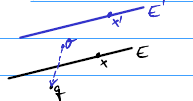
\includegraphics[width=3cm,height=2cm]{bild 2.9}
\end{figure}\\
\textbf{2.10\underline{Bsp.:}} Abstand von q = $\begin{pmatrix}
	1\\-2
\end{pmatrix} zu H_{\begin{pmatrix}
	2\\3
\end{pmatrix},5} =\{\begin{pmatrix}
	x\\y
\end{pmatrix} \in \mathbb{R}^2;2x+3y=5\}$ist\\
\begin{equation}
	\frac{|\textless q,c 
	\textgreater-\alpha|}{||c||}=\frac{|1\cdot2+(-2)\cdot3-5|}{\sqrt{2^2+3^2}}=
	\frac{|2-6-5|}{\sqrt{13}}=\frac{9}{\sqrt{13}}.
\end{equation}
\hfill$\square$\\
\textbf{2.11\underline{geometrische Anschauung von 
Funktionen}}$f:D\rightarrow\mathbb{R}^m$ mit $ \varnothing \neq D \subseteq 
\mathbb{R}^n,m,n\in\mathbb{N}.$\\
Der \ul{Graph von f} ist \setulcolor{yellow}
\begin{align}
	\text{\ul{G(f)}}:&=\{(x,f(x))\in \mathbb{R}^{n+m};x\in D\}\\
	&=\{(\xi_1,...,\xi_n,f(\xi_1,...,\xi_m));(\xi_1,...,\xi_n)^T\in D\}\subseteq 
	\mathbb{R}^{n+m},
\end{align}
wir "verkleben" die Koordinaten von x mit denen von f(x) zu Vektoren 
im$\mathbb{R}^{n+m}$.\\
\underline{(1)Fall m=1}, d.h. eine $\mathbb{R}$-wertige/reellwertige Funktion, 
auch \setulcolor{red} \ul{Skalarfeld} genannt.\\
Für n=2 läßt sich G(f) oftmals als "Fläche" im$\mathbb{R}^3$ deuten, für die 
man bei festen $c \in \mathbb{R}$ die \ul{"Niveaulinie" ${x\in D;f(x)=c}$ vom 
Niveau c} betrachten kann (wie Höhenlinien bei Wanderkarten).\\
Dabei macht man "Horizontalschnitte", d.h man schneidet den Graphen G(f) mit 
der Ebene
der Glg. $\xi_3= c(d.h"z=c")$ und projiziert den Schnitt auf die 
$\xi_1-\xi_2$-Ebene (bzw. xy-Ebene).\\
(a)\underline{Bsp.:} Für die Halbkugelfläche $f:\{(x,y); x^2+y^2\leq 
1\}\rightarrow\mathbb{R}, (x,y)\rightarrow \sqrt{1-x^2-y^2}\\$
Sind die Niveaulinien\\
\begin{equation}
	\text{von Niveau c:}\begin{cases}
		\emptyset, & c>0,c<0\\
		\{0\}, & c=1\\
		\{x,y\}\in \mathbb{R}^2;x^2+y^2=1-c^2, & 0\leq c<1\leftarrow Kreise vom 
		radius\sqrt{1-c}
	\end{cases}
\end{equation}
$\leadsto G(f)=?$\redcircle{Ü}\\
(b) \underline{Bsp.:} $f:\mathbb{R}^n\rightarrow\mathbb{R}$ affin-Linear, d.h.
$f(\xi_1,...,\xi_n)[$Eigentlich$: f\begin{pmatrix}
	\xi_1\\
	\vdots\\
	\xi_n
\end{pmatrix}]= \alpha_1\xi_1+...+\alpha_n\xi_n+\beta$
mit $\alpha_1,...,\alpha_n, \beta\in\mathbb{R}$. Der Graph 
G(f)$=\{(\xi_1,...,\xi_n,ß+\sum_{i=1}^{n}\alpha_i\xi_i)^T;\xi_1,...,\xi_n\in\mathbb{R}\}\subseteq\mathbb{R}^{n+1}$
ist (i.a) eine n-dim Hyperebene im $\mathbb{R}^{n+1}$ mit der Gleichung 
$-\sum_{i=1}^{n}\alpha_i\xi_i+\xi_{n+1}=ß$.\\
(c) Die Schnitte des Graphen G(f) einer Fkt. $f:\mathbb{R}^n\rightarrow 
\mathbb{R}$ mit den Koordinatenhyperebenen, die jeweils durch eine Glg. 
$\xi_i=0,1\leq i\leq n$, gegeben sind, sind "Vertikalschnitte". Bei n=2 hat man 
da die xy - Ebene der Glg. z=0, die xz-Ebeene der Glg. y=0, und x=0 ist die 
yz-Ebene, die zu geh. Vertikalschnitte sind ${(x,y,0)^T; f(x,y)=0}, 
\{(x,0,f(x,0))^T;x\in \mathbb{R}\}, \{(0,y,f(0,y))^T;y\in\mathbb{R}\}.$\\
\\
(2)\underline{Fall n=m:} $f: D\rightarrow \mathbb{R}^n$ mit $ D \subseteq 
\mathbb{R}^n$ heißt \ul{Vektorfeld.}\\
(3)\underline{Fall n=1:} Etwa $f:I\rightarrow\mathbb{R}^m$, wo $I \subseteq 
\mathbb{R}^1$ ein Intervall ist. Der Graph ist ein "Kurvenähnliches" Gebilde in 
$\mathbb{R}^{1+n}$, die Funktionswerte in $\mathbb{R}^m$ können mit der 
Projektionsalb, $pr_i:\mathbb{R}^m\rightarrow\mathbb{R}$ aus \setulcolor{blue} 
\ul{1.11} Komponentenweise betrachtet werden durch $f_i:= pr_i\circ 
f,f_i:I\rightarrow\mathbb{R}$ für $1\leq i\leq m$.\\
Diese Funktionen können mit den Methoden der Analysis I untersucht werden, z.b 
Untersuchung auf Differenzierbarkeit (f ist diffbar, wenn alle $f_i$ diffbar, 
sodass wir in diesem Fall von einer \setulcolor{red}\ul{Kurve} sprechen wollen, 
vgl. \setulcolor{blue}\ul{4.5}).\\
\\
\textbf{2.12\underline{Def.:}} Sind $pr_1,...,pr_m$ die Projektionsabb. 
$\mathbb{R}^m\rightarrow\mathbb{R}$, und $f: D\rightarrow\mathbb{R}^m, 
D\subseteq\mathbb{R}^n$, dann heißt \setulcolor{red}\ul{$f_i:=pr_i\circ f$} 
$:D\rightarrow\mathbb{R}$ die \ul{i-te Komponentenfunktion (auch 
Koordinatenfunktion) von f}, wo $1\leq i \leq m$ ist. Damit gilt 
$f(x)=\begin{pmatrix}
	f_1(x)\\f_2(x)\\\vdots\\f_m(x)
\end{pmatrix}
\in \mathbb{R}^m$.\\
Viele Eigenschaften von Funktionen f mit $\mathbb{R}^m$ als Zielmenge können 
mit ihren Komponentenfunktionen (leichter) untersucht werden, da diese 
Skalarfelder sind.\\
\\
\textbf{2.13\underline{Bsp.:}} Sei $f:\mathbb{R}^n\rightarrow\mathbb{R}^m$ eine 
Lineare Abb. (im Sinne der Linearen Algebra),\\
also $f(x)= A\cdot x$ mit einer Matrix $A\in \mathbb{R}^{mxn}$, etwa 
$A=(\alpha_{ij})$.\\
Die m Komponentenfkt. sind $f_i:\mathbb{R}^n\rightarrow\mathbb{R}, 
f_i(x)=\sum_{j=1}^{n}\alpha_{ij}\xi_j$, wo $1\leq i\leq m$.\\
Der Graph jeder einzelnen Komponentenfunktion ist (i.a.) eine Hyperebene im 
$\mathbb{R}^{n+1}$ mit der Gleichung $\xi_{n+1}=\sum_{j=1}^{n}a_{ij}\xi_j$, und 
der Gesamtgraph G(f) Wird durch die m Gleichungen 
$\xi_{n+i}=\sum_{j=1}^{n}a_{ij}\xi_j$ beschrieben.


\end{document}
